\documentclass[11pt]{article}

\usepackage{amsmath}
\usepackage{booktabs}
\usepackage{enumitem}
\usepackage[T1]{fontenc}
\usepackage[margin=1in]{geometry}
\usepackage{graphicx}
\usepackage[utf8]{inputenc}
\usepackage{libertine}
\usepackage[libertine]{newtxmath}

\title{MATH 114 Final Exam Question 6}
\author{Brandon Tsang}
\date{April 14, 2020}

\begin{document}
    \maketitle
    \begin{enumerate}[label=\textbf{\arabic*.}, start=6]
        \item{
            \textbf{\boldmath Consider the following diagram, which is generated by a matrix \(M\):}
            \begin{center}
                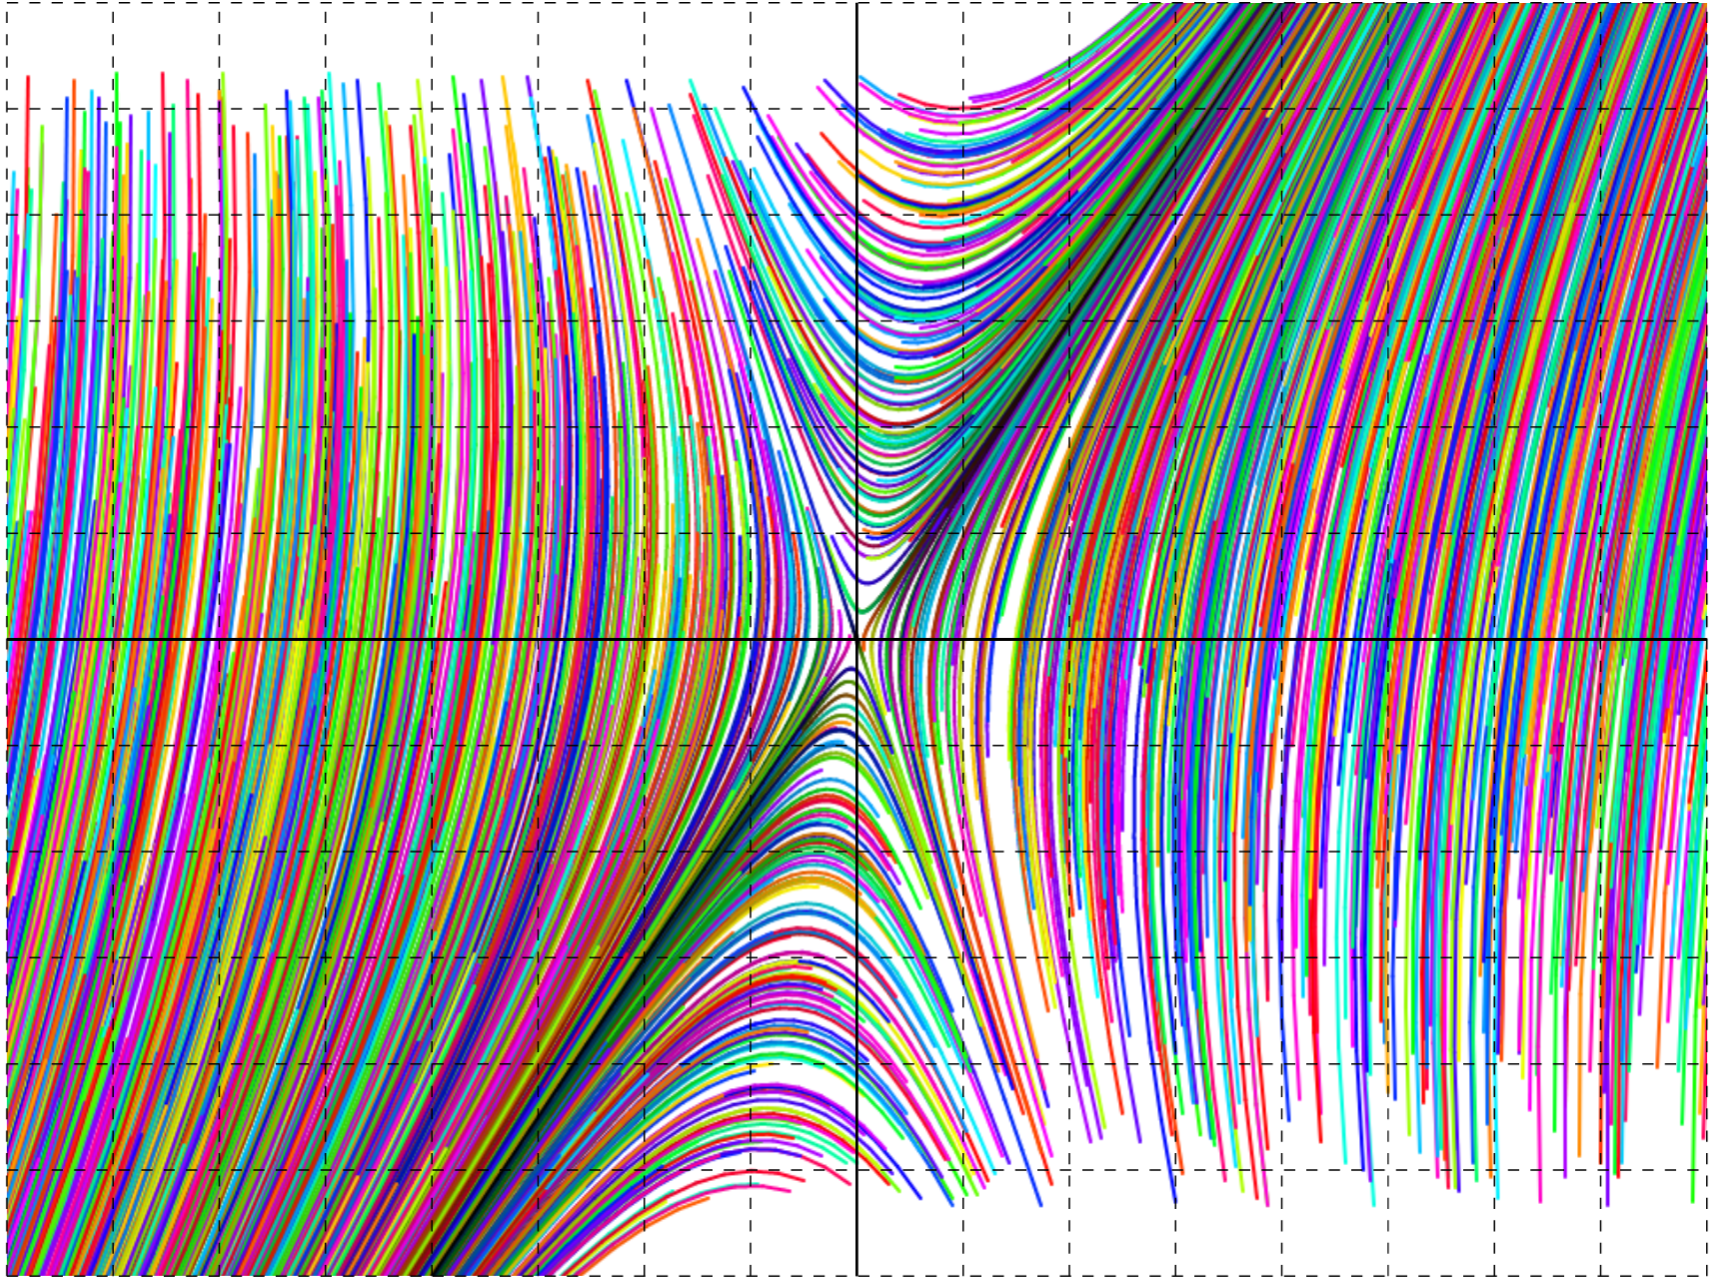
\includegraphics[width=0.8\linewidth]{q6.png}
            \end{center}
            \begin{enumerate}[label=\textbf{(\alph*)}]
                \item{
                    \textbf{\boldmath What can you say about \(M\)? Include as much detail as you can.}
                    \par
                    \(M\) has two eigenvalues, with their associated eigenvectors lying on the ``asymptotes'' in the image. This comes from the fact that \(M\)'s eigenvectors will only be scaled up or down in its transformation. This corresponds to straight lines on the image.
                    \par
                    \(\det(M)>1\), since all of the vectors transform away from the origin.
                }
                \pagebreak
                \item{
                    \textbf{\boldmath Consider the following diagram, which is generated by a matrix \(N\):}
                    \begin{center}
                        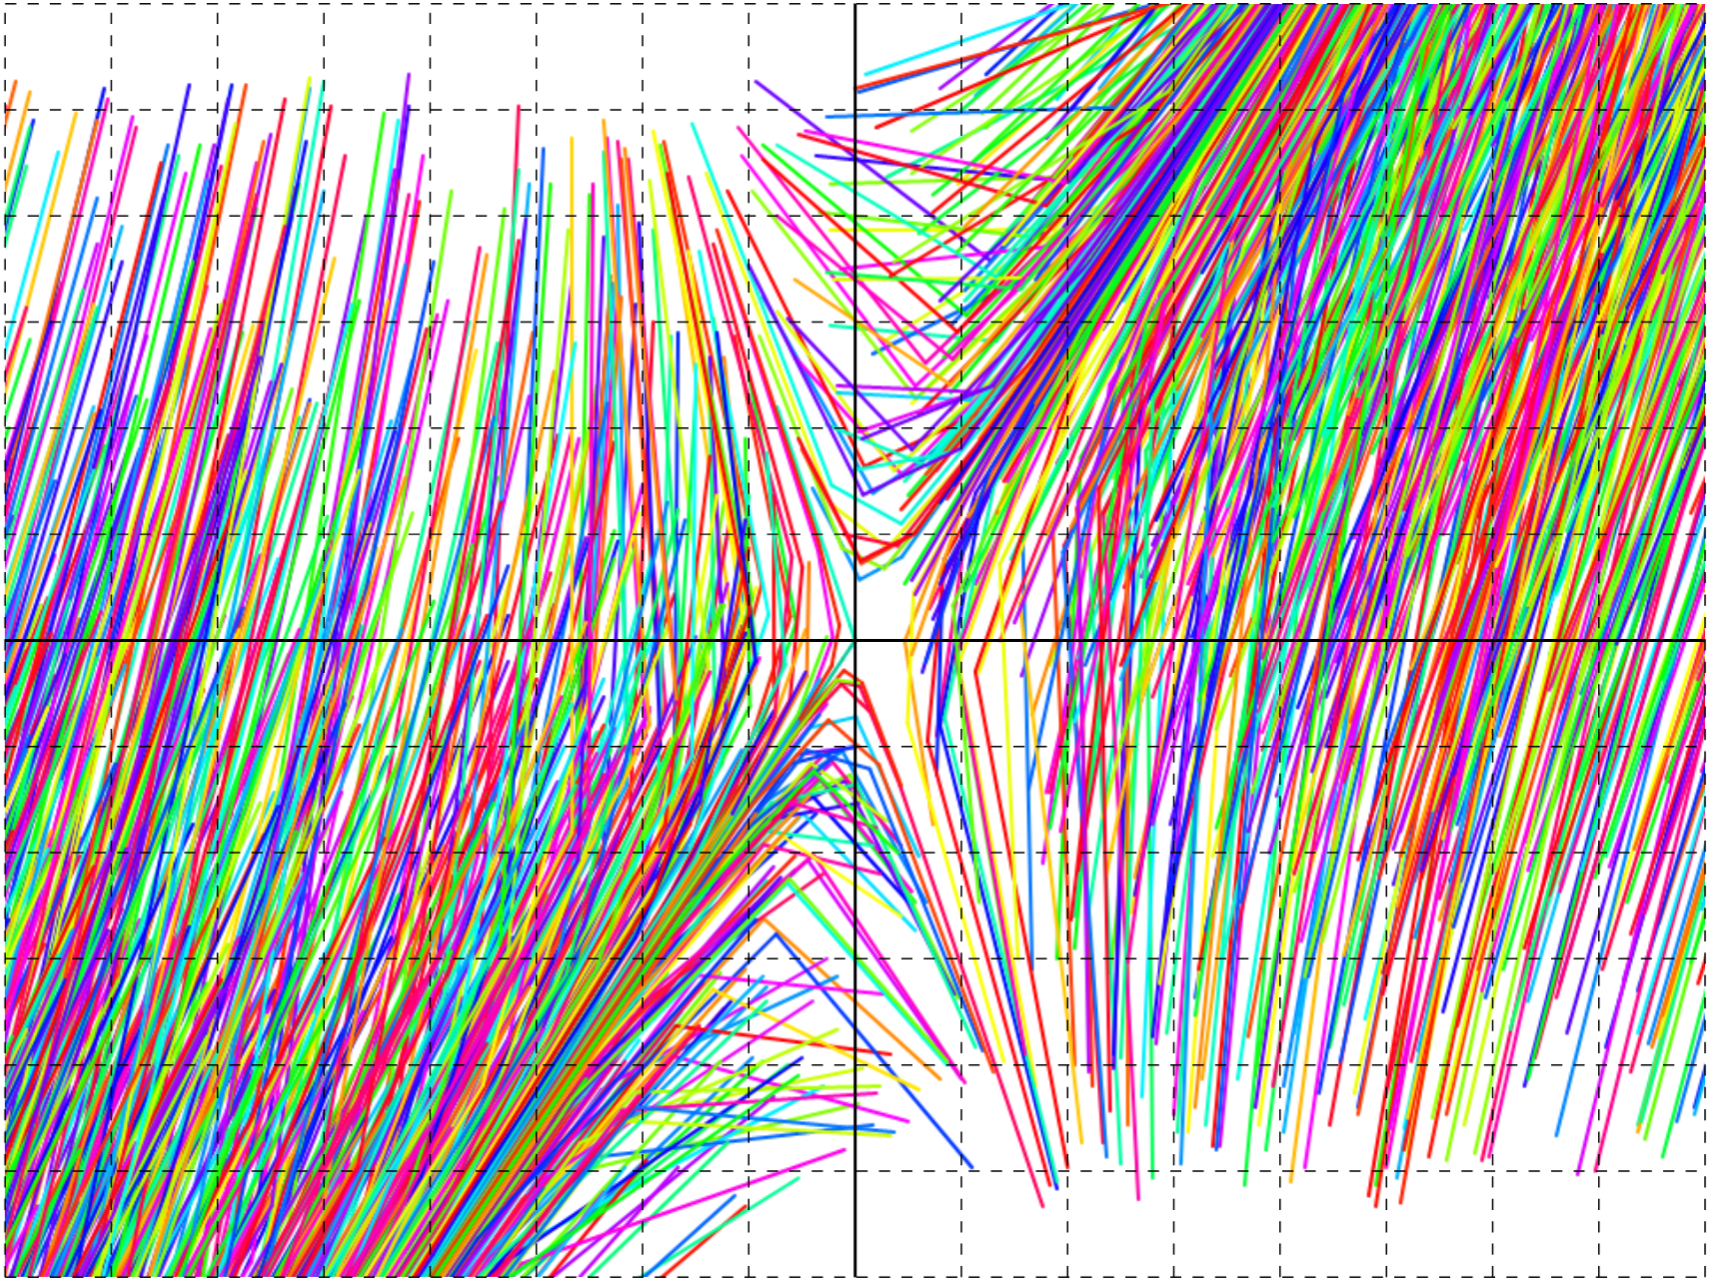
\includegraphics[width=0.8\linewidth]{q6b.png}
                    \end{center}
                    \textbf{\boldmath \(M\) and \(N\) are similar. What is the same about \(M\) and \(N\)? What is different about \(M\) and \(N\)?}
                    \par
                    \(M\) and \(N\) both share the same characteristics as I mentioned above. However, the lines created by \(N\) are much more jagged than those created by \(M\). This means that \(N\) transforms vectors more than \(M\) does. In mathematical terms, this means that \(\det(N)>\det(M)\). In fact, \(N\) is likely a scalar multiple of \(M\).
                }
            \end{enumerate}
        }
    \end{enumerate}
\end{document}
